\documentclass[parskip=full]{scrartcl}

\usepackage[utf8]{inputenc}			% Umlaute, Sonderzeichen
\usepackage[ngerman]{babel}			% deutsche Sprache
\usepackage[tocfullflat]{tocstyle}			% Inhaltsverzeichnis
\usepackage{enumitem}				% Listen
\usepackage{graphicx}					% Grafiken
\usepackage{hyperref}					% Hyperlinks
\usepackage[nonumberlist]{glossaries}		% Glossar

\makenoidxglossaries

\newglossaryentry{bsp}{name=Beispiel, description=Beispieleintrag}

\subject{Pflichtenheft}
\title{Visuelle Programmiersprache für den Physikunterricht zur Datenerfassung auf einem Raspberry Pi}
\subtitle{Version 0.1.1}
\author{David Gawron \and Stefan Geretschläger \and Leon Huck \and Jan Küblbeck \and Linus Ruhnke}
\date{\today}

\begin{document}

\maketitle

\newpage

\tableofcontents 					% generate pdf twice to update

\section{Produktübersicht}



\section{Zielbestimmung}

Die Anwendung soll es Lehrern ermöglichen, Schülern ab der siebten Klasse Grundkenntnisse der digitalen Messwerterfassung in einer für Schüler interessante und motivierenden Weise näher zu bringen. Dabei werden technische Details, wie Konfigurationsdateien, vor dem Schüler verborgen. Damit wird der Schüler nicht überfordert, sondern soll ermutigt werden, selbstständig mit der Software umzugehen. Dabei wird ihm die Grundkenntnisse von Ursache und Wirkung durch spaßige Messungen demonstriert.
\newline 
Es wird eine graphische Oberfläche angeboten, die es dem Schüler ermöglicht allein per Drag and Drop eine Messanordnung zu erstellen. Die Details die dahinter stecken sind vor dem Schüler verborgen. Die Anwendung motiviert den Schüler dazu mit Sensoren, Transformationen und Darstellungen zu spielen und Dinge auszuprobieren. Dabei wird ihm durch eine intuitive Status- und Fehleranzeige gezeigt, ob seine Konstruktion funktioniert. Wenn nein, dann zeigt sie ihm an, wo das Problem liegt und warum es nicht funktioniert. Eine lästige Fehlersuche bleibt dem Schüler dann erspart.
\newline
 Außerdem liefert die Anwendung dem Schüler zu den vorhandenen Bausteinen und zu der Anwendung allgemein die nötigen Informationen die er für die Nutzung braucht. Dabei wird auf ein ausführliches Tutorial am Anfang verzichtet. Die Anwendung liefert die Informationen häppchenweise durch Informationsanzeigen an den jeweilig relevanten Stellen. Damit findet der Schüler die Hilfe die er sucht an der Stelle an der er sie braucht. 
\newline
Die Anwendung ermöglicht es dem Lehrer vor dem Unterricht eine Reihe von Messversuchen teilweise oder ganz zu konfigurieren und zu speichern. Dabei kann er genau bestimmen was er den Schülern zeigen will. Diese Konfigurationen kann er dann schnell und einfach im Unterricht zum Einsatz bringen.
\newline  
Weiter ermöglicht es die Anwendung, dass Schüler aus höheren Klassen mit mehr Details der digitalen Messwerterfassung zusammen gebracht werden. Diese nutzen keine oder nur eine kleine vorgefertigte Konfiguration. Sie können dann auch selbst einen Sensor konfigurieren. Trotz des höheren Detailgrads bleibt die Anwendung übersichtlich und strukturiert. Damit bleiben auch komplexere Messversuche für den Schüler motivierend.
\newline

Die Anwendung ist als Schnittstelle zwischen PhyPiDAQ und dem Nutzer zu verstehen. Sie ermöglicht dem Nutzer über eine übersichtliche, strukturierte und intuitive GUI sowie über eine einfache Bedienung die Nutzung eines Raspberry Pi mit PhyPiDAQ. Dadurch soll dem Schüler digitale Messwerterfassung, Physik und auch Informatik in einer motivierenden Weise näher gebracht werden. Womöglich kann die Anwendung den Schüler auch für diese Themen begeistern.  

\subsection{Musskriterien}

\begin{itemize}

\item Datenhandhabung
\begin{itemize}

\item Der Benutzer kann Ergebnisse aus einer Messung speichern und laden.
\item Der Benutzer kann gleichzeitig Daten aus einer Messung darstellen und diese Daten auch weiter verwenden.
\item Der Benutzer kann eine Messkonfiguration speichern und laden.
\item Der Benutzer kann die Anwendung nutzen, ohne persönliche Daten preiszugeben.

\end{itemize}



\item Benutzbarkeit der GUI
\begin{itemize}

\item Die Anwendung reagiert auf Veränderungen so schnell, dass das Prinzip von Ursache und Wirkung intuitiv erfahren werden kann.
\item Der Benutzer kann Komponenten einer Messkonfiguration per Drag and Drop hinzufügen.
\item Der Benutzer kann Komponenten intuitiv mit einander verbinden.
\item Die Anwendung lässt sich mit dem Wissen eines Schülers aus der siebten Klasse bedienen.
\item Die Anwendung lässt sich auch mit einer rot-grün-Schwäche komplett nutzen.

\end{itemize}

\item Funktionen
\begin{itemize}

\item Die Anwendung erhält Daten durch den Raspberry Pi mit PhyPiDAQ oder aus einer Datei und kann diese dann transformieren und darstellen.
\item Die Anwendung enthält vorgefertigte Standardelemente, wie z.B. to do
\item Die Anwendung enthält vorgefertigte Standardkonfigurationen.

\end{itemize}

\item Information und Rückmeldung
\begin{itemize}

\item Ist ein verwendeter Sensor nicht angeschlossen oder fehlerhaft, meldet die Anwendung dies über eine Pop-Up-Nachricht.
\item Die Anwendung enthält Erklärungen und Informationen zu den einzelnen Komponenten, d.h. zu den Sensoren, Transformationen und Darstellungen.
\item Die Anwendung enthält Erklärungen und Informationen zu den GUI-Bereiche, d.h. zu dem Auswahlbereich der Komponenten, zu dem Messversuchsbereich und zu dem Anzeigebereich.
\item Falls nicht alle Kanäle verbunden sind, meldet die Anwendung dies dem Benutzer mit einer Fehlermeldung, falls dieser versucht die Messung zu starten. 

\end{itemize}

\item Sonstiges
\begin{itemize}

\item Die Anwendung kommuniziert mit den Nutzer auf deutsch.
\item Die Anwendung soll auf die Unterstützung neuer Sensoren erweiterbar sein.
\item Die Anwendung hält die Datenschutzrichtlinie "`to do"' ein.
\item Die Anwendung hält die Schulrichtlinie "`to do"' ein.

\end{itemize}

 \end{itemize}

\subsection{Sollkriterien}

\begin{itemize}

\item Die Anwendung soll auf die Erstellung eigener Transformationen erweiterbar sein.
\item Die Anwendung soll auf andere Sprachen erweiterbar sein.
\item Die Anwendung soll allein auf dem Raspberry Pi laufen können.
\item Farbkodierung der GUI-Elemente
\item Einfache Erweiterbarkeit
\subitem Einheitliches Interface für Sensoren


 \end{itemize}

\subsection{Wunschkriterien}

\begin{itemize}

\item Übertragung der Messdaten über Netzwerkschnittstelle
\item Spiele, „nachmachen“ von vorgegebenen Messergebnissen
\item Ausfürliche Beschreibung der physikalische Hintergründe

 \end{itemize}

\subsection{Abgrenzungskriterien}

\begin{itemize}

\item Unterschiedliche Benutzerkonten sind nicht zu implementieren
\item Personenbezogene Daten werden nicht gespeichert

 \end{itemize}

\section{Produkteinsatz}

\begin{itemize}

\item Anwendungsbereich: Die Software wird durch Schulen in Deutschland auf schuleigener Hardware eingesetzt.
\item Zielgruppe: Lehrer und Schüler ab der 7. Klasse.
\item Betriebsbedingungen: TODO

\end{itemize}

\section{Produktumgebung}

Die Anwendung läuft auf einem Computer, die Messdaten werden über Messsensoren an einem Raspberry Pi erfasst.

\subsection{Software}

Die Anwendung läuft auf Computern mit den Betriebssystemen Linux ab Kernel 7 und Microsoft Windows ab Windows 7 oder neuer. Die Anwendung muss auf dem Computer vollständig installiert sein. 

\subsection{Hardware}

Die Anwendung läuft auf gewöhnlichen Computern.
Auf dem per USB-Schnittstelle verbundenen Raspberry Pi muss PhyPi DAQ installiert und verwendungsfähig sein.
Die an das Raspberry Pi angeschlossenen Messsensoren müssen richtig und sinnvoll angeschlossen sein.

\subsection{PhyPiDAQ}

Bei PhyPiDAQ\footnote{\url{https://github.com/GuenterQuast/PhyPiDAQ}} handelt es sich um eine Anwendung zur Datenerfassung und Analyse mit einem Raspberry Pi. Diese ist nicht Bestandteil des Produktes, wird jedoch zur Datenerfassung und Datenverarbeitung und somit zur Funktionalität der Anwendung  benötigt. Das Programm, welches in der Programmiersprache python3 geschrieben ist bietet einfache und einheitliche Schnittstellen zur Verwendung der Messsensoren.

\section{Funktionale Anforderungen}

\subsection{GUI}

\begin{itemize}
\item[F010] Die Benutzer erreichen nach Öffnung der Anwendung direkt die GUI.
\item[F020] Der Benutzer öffnet durch den Einstellungen-Button die Einstellungen.
\item[F030] Der Benutzer kann durch den Datei-Button die Dateiverwaltung öffnen.
\item[F040] Der Benutzer kann durch den Hilfe-Button das Hilfe Fenster öffnen.
\end{itemize}

\subsubsection{Menüfeld}

\begin{itemize}
\item[F050] Der Benutzer öffnet durch den Sensoren-Button die Auswahl an Sensoren.
\item[F060] Der Benutzer öffnet durch den Verbindungen-Button die Auswahl an Verbindungen.
\item[F070] Der Benutzer öffnet durch den Darstellungen-Button die Auswahl an Darstellungen.
\item[F080] Der Benutzer erhält durch verschiedene Farben der Konfigurationsbausteine eine visuelle Repräsentationen ihrer Komplexität.
\end{itemize}

\subsubsection{Optional: Zusätzliche Funktionen im Menüfeld}

\begin{itemize}

\item[F090] Der Benutzer kann durch den Sensoren hinzufügen-Button weitere Sensoren hinzufügen.
\item[F100] Der Benutzer kann durch den Transformationen hinzufügen-Button weitere Transformationen hinzufügen.
\item[F110] Die in Transformationen in F100 sollen in eigenen Python-Skripten geschrieben werden.
\end{itemize}

\subsubsection{Konfigurationsfeld}

\begin{itemize}
\item[F120] Durch Drag und Drop kann der Benutzer Konfigurationsbausteine im Konfigurationsfeld platzieren.
\item[F130] Durch Betätigen des Messung starten-Button startet der Nutzer eine Messung.
\end{itemize}

\subsubsection{Darstellungsfenster}

\begin{itemize}
\item[F140] Das Darstellungsfenster ist bei der Initialisierung der Anwendung leer.
\item[F150] Durch die Benutzerkonfiguration im Konfigurationsfeld wird durch F90 automatisch die Darstellungsart im Darstellungsfenster geöffnet.
\end{itemize}

\subsection{Konfigurationserstellung}

\begin{itemize}

\item[F160] Über F30 kann der Benutzer gespeicherte Standartkonfigurationen öffnen oder alte Messwerte verwenden.
\item[F170] Durch F160 geladene Konfigurationen und Messdaten werden automatisch nach Format überprüft.
\item[F180] Aus F50 kann der Benutzer Sensoren durch Drag und Drop in das Konfigurationsfeld ziehen.
\item[F190] Die Anwendung sollte automatisch überprüfen, ob der ausgewählte Sensor richtig angeschlossen ist.
\item[F200] Die Anwendung gibt durch F190 automatisch eine visuelle Rückmeldung über die Farbe des Sensors.
\item[F210] Aus F60 kann der Benutzer eine oder mehrere Verbindungen durch Drag und Drop in das Konfigurationsfeld ziehen.
\item[F220] Die ausgewählten Verknüpfungen kann der Benutzer mit einem ausgewählten Sensor verknüpfen.
\item[F230] Die Anwendung sollte automatisch überprüfen, ob die Verbindungen eine geeignete Kombination mit dem Sensor darstellt.
\item[F240] Aus F70 kann der Benutzer eine Darstellungsart per Drag und Drop in das Konfigurationsfeld zu ziehen.
\item[F250] Die Ausgewählte Darstellung kann der Benutzer mit einer Verbindung verknüpfen.
\item[F260] Die Anwendung sollte automatisch überprüfen, ob die gewählte Darstellungsart eine sinnvolle Repräsentation der Messdaten darstellt.
\item[F270] Über F30 kann der Benutzer seine eigene Konfiguration über einen Konfiguration speichern- Knopf speichern.
\item[F280] Bausteine die ein Benutzer nicht mehr in dem Konfigurationsfeld haben möchte können durch Drag und Drop in die Menüleiste wieder versteckt werden.

\end{itemize}

\subsection{Messablauf}

\begin{itemize}

\item[F290] Die Anwendung sollte dem Benutzer erlauben den Wertebereich und die Dauer der Messung festzulegen.
\item[F300] Der Nutzer kann durch F90 die Messung nach der Benutzerkonfiguration starten.
\item[F310] Durch F300 wird automatisch mit der visuellen Darstellung der Messdaten begonnen.
\item[F320] Der Nutzer kann durch den Messung Messung löschen-Button eine durchgeführte Messung pausieren und die visuelle Darstellung auf den Ausgangszustand bringen.
\item[F330] Durch F320 wird nicht die Benutzerkonfiguration gelöscht.
\item[F340] Durch F320 muss der Benutzer erst die Messung starten um weiter zu messen.
\item[F350] Der Benutzer kann durch den Messung pausieren-Button die Messung pausieren.
\item[F360] Der Benutzer kann durch den Messung-fortsetzen-Button die Messung fortsetzen.
\item[F370] Der Benutzer kann eine Messung durch F310 nur fortsetzen, wenn sie zuvor durch F300 pausiert wurde.
\item[F380] Der Benutzer kann durch den Messdaten speichern-Button die gemessenen Daten speichern.
\item[F390] Der Benutzer kann durch den Graph speichern-Button den durch die Messung erzeugten Graphen speichern.
\item[F400] Bei F370 und F380 öffnet sich automatisch das Verzeichnis und der Nutzer muss einen eigenen Dateinamen eingeben und speichern. 

\end{itemize}

\subsection{Fehlermeldungen}

\begin{itemize}
\item[F410] Durch F130 geladene Konfigurationen und Messdaten werden automatisch nach Format überprüft und eine aussagekräftige Fehlermeldung zurückgegeben.
\item[F420] Durch F190 und F220 wird bei einer ungültigen Kombination von zwei Konfigurationsbausteinen eine aussagekräftige Fehlermeldung zurückgegeben
\item[F430] Die Anwendung sollte dem Benutzer automatisch durch Pop-Up Benachrichtigung darauf hinweisen, dass bei Betätigen des Messung löschen-Button oder bei Schließen der Anwendung die Messdaten ohne vorheriges Betätigen des Messdaten speichern-Button verloren gehen.

\end{itemize}

\subsection{Bedienungshilfen}

\begin{itemize}

\item[F440] Bei enthaltenen Konfigurationsbausteine sollen einen Information-Button besitzen, über welche der Benutzer Informationen und Hilfestellung bereitgestellt bekommt.
\item[F450] Über den Hilfe-Button erhält der Nutzer eine kurze Beschreibung zur Funktionalität der Anwendung.

\end{itemize}

\subsection{Sprache}

\begin{itemize}

\item[F450] Die Anwendung ist in deutscher Sprache.

\end{itemize}

\subsubsection{Optional: Internationalisierung}

\begin{itemize}

\item[F460] Die Anwendung stellt dem Benutzer weitere Sprachpakete für die GUI zur Verfügung.
\item[F470] Durch F20 ist die Sprache für den Nutzer änderbar.

\end{itemize}

\subsection{Sonstiges}

\begin{itemize}

\item[F480] Die in der Anwendung enthaltenen Farben sollten mit Rücksicht auf Benutzer mit Rot-Grün Schwäche oder Farbenblindheit ein barrierefreies Verwendung der Anwendung ermöglichen.

\end{itemize}

\subsubsection{Optional: Sonstiges}

\begin{itemize}

\item[F490] Durch F20 sollte der Benutzer die in der Anwendung verwendeten Farben ändern können.
\item[F500] Durch F20 sollte der Benutzer die in der Anwendung verwenden Buchstabengröße verändern können.

\end{itemize}

\subsection{Schnittstelle}

\begin{itemize}
\item just a test

\end{itemize}

\section{Produktdaten}

Zu speichern sind ausschließlich:

\begin{itemize}

\item Konfigurationsdaten
\item Physikalische Messdaten

\end{itemize}

Es sollen keine benutzer- oder personenbezogenen Daten gespeichert werden.

\section{Nichtfunktionale Anforderungen}

\subsection{Produktleistungen}

\begin{itemize}

\item[NF010] Auslesen von Sensordaten innerhalb von (5?) ms. //TODO PhyPiDAQ Abhängigkeit
\item[NF015] Alle (5?) ms können neue Daten angefordert werden.
\item[NF020] Verarbeitung ausgelesener Daten innerhalb von 10 ms.
\item[NF030] Bis zu drei Sensoren können zeitgleich verwendet werden.
\item[NF040] Bis zu (6?) Transformationen können hintereinander verbunden werden.
\item[NF050] Bis zu (3?) Senken können zeitgleich verwendet werden.

\end{itemize}

\subsection{Benutzbarkeit}

\begin{itemize}

\item[NF060] Die Benutzeroberfläche ist für Siebtklässler verständlich.
\item[NF070] Ungespeicherte Daten werden nicht ohne Warnung verworfen.
\item[NF080] Programmfehler werden dem Benutzer gegenüber klar kommuniziert.
\item[NF090] Schriftgröße von Text kann verändert werden.
\item[NF100] Farbschema von farbigen UI-Elementen ist veränderbar.

\end{itemize}

\subsection{Zuverlässigkeit}

\begin{itemize}

\item[NF110] Die Anwendung reagiert konsistent auf Eingaben.
\item[NF120] Unerwartete und fehlerhafte Eingaben führen nicht zum Systemabsturz.
\item[NF130] Verbindungsverlust von Sensoren führt dies nicht zum Systemabsturz.

\end{itemize}

\subsection{Sonstige}

\begin{itemize}

\item[NF210] Die Software ist vollständig quelloffen und frei.\footnote{\url{https://www.gnu.org/philosophy/free-sw.de.html}}
\item[NF220] Die Datenschutz-Grundverordnung wird nicht verletzt.

\end{itemize}

\section{Globale Testfälle und Testszenarien}

\begin{itemize} 

\item[T010] to do Benutzung des Startbildschirms
\begin{itemize}

\item []\textbf{Stand} 
\item []\textbf{Aktion} 
\item []\textbf{Reaktion} 

\end{itemize}


\item[T020] drag and drop Sensor
\begin{itemize}

\item []\textbf{Stand} Offenes Fenster der Hauptanwendung.
\item []\textbf{Aktion} Der Benutzer öffnet das gewünschte Tab und zieht einen Sensor in die Konstruktionsfläche in die Mitte und lässt es dort los.
\item []\textbf{Reaktion} Das Icon des Sensors bleibt als Kopie auf der Konstruktionsfläche erhalten.

\end{itemize}

\item[T025] to do Überprüfung T020
\begin{itemize}

\item[]\textbf {Stand} 
\item[]\textbf{Aktion} 
\item[]\textbf{Reaktion} 

\end{itemize}

\item[T030] drag and drop Transformation und Überprüfung
\begin{itemize}

\item []\textbf{Stand} Offenes Fenster der Hauptanwendung.
\item []\textbf{Aktion} Der Benutzer öffnet das Tab der Transformationen und zieht eine Transformation in die Konstruktionsfläche in die Mitte und lässt sie dort los.
\item []\textbf{Reaktion} Das Icon der Transformation bleibt als Kopie auf der Konstruktionsfläche erhalten. 

\end{itemize} 

\item[T035] to do Überprüfung T030 automatisch

\item[T040] drag and drop einer Darstellung und deren Überprüfung
\begin{itemize}

\item []\textbf{Stand} Offenes Fenster der Hauptanwendung.
\item []\textbf{Aktion} Der Benutzer öffnet das Tab der Darstellung und zieht eine Darstellung in die Konstruktionsfläche in die Mitte und lässt sie dort los.
\item []\textbf{Reaktion} Das Icon der Darstellung bleibt als Kopie auf der Konstruktionsfläche erhalten. 

\end{itemize}

\item[T045] to do Überprüfung T040 automatisch

\item[T050] Einstellen von Messbereich und Dauer einer Messung
\begin{itemize}

\item[1.]\textbf {Stand} Offenes Fenster der Hauptanwendung.
\item[]\textbf{Aktion} Der Benutzer drückt auf den "`Anpassen"' Knopf.
\item[]\textbf{Reaktion} Das Fenster zum Anpassen der Messung öffnet sich.

\item[2.]\textbf {Stand} Offenes Fenster zum Anpassen der Messung.
\item[]\textbf{Aktion} Der Benutzer veränderet die Einstellungen und drückt dann auf den "`OK"' Knopf.
\item[]\textbf{Reaktion} Die Einstellungen werden übernommen. Das Fenster zum Anpassen der Messung schließt sich.

\end{itemize}

\item[T060] Aufrufen von Informationen
\begin{itemize}
\item[]\textbf {Stand} Offenes Fenster der Anwendung.
\item[]\textbf{Aktion} Der Benutzer drückt auf einen "`I"' Knopf.
\item[]\textbf{Reaktion} Ein Informationsfenster mit den zugehörigen Informationen öffnet sich.
\end{itemize}

\item[T070] Lade Datei als Quelle und Überprüfung
\begin{itemize}

\item[1.]\textbf {Stand} Offenes Fenster der Hauptanwendung.
\item[]\textbf{Aktion} Der Benutzer drückt auf den "`lade von Datei"' Knopf.
\item[]\textbf{Reaktion} Ein Fenster zum Auswählen eines Pfades öffnet sich.

\item[2.]\textbf {Stand} Offenes Fenster Auswählen eines Pfades.
\item[]\textbf{Aktion} Der Benutzer wählt einen Pfad zu einer gültigen Datei als Quelle aus. Danach drückt er auf den "`Laden"' Knopf.
\item[]\textbf{Reaktion} Die Daten werden als Sensor Icon zu den verfügbaren Sensoren hinzugefügt.

\end{itemize}

\item[T090] Laden einer Messung
\begin{itemize}

\item[1.]\textbf {Stand} Offenes Fenster der Hauptanwendung.
\item[]\textbf{Aktion} Der Benutzer drückt auf den "`Laden"' Knopf.
\item[]\textbf{Reaktion} Das Fenster zum Laden eines Versuchs öffnet sich.

\item[2.]\textbf {Stand} Offenes Fenster zum Laden.
\item[]\textbf{Aktion} Der Benutzer gibt den Speicherort einer gültigen Versuchsdatei an. Dann drückt der Benutzer auf den "`Laden"' Knopf.
\item[]\textbf{Reaktion} Der Versuch wird geladen. Das Fenster zum laden schließt sich. In der Konstruktionsfläche wird der Versuch dargestellt.

\end{itemize}

\item[T100] Starten einer Messung
\begin{itemize}
\item[]\textbf {Stand} Offenes Fenster der Hauptanwendung mit einem gültigen Aufbau in der Konstruktionsfläche.
\item[]\textbf{Aktion} Der Benutzer drückt auf den "`Start"' Knopf.
\item[]\textbf{Reaktion} Das Konstruktionsfenster wird vor Veränderung geschützt. Die Anzeigefläche rechts stellt die gewünschten Darstellungen dar. Falls ein Sensor nur endlich viele Werte eingeben soll, pausiert sich das Programm automatisch danach.
\end{itemize}

\item[T110] to do
\begin{itemize}

\item[]\textbf {Stand} 
\item[]\textbf{Aktion} 
\item[]\textbf{Reaktion} 

\end{itemize}

\item[T115] Zurücksetzen einer Messung
\begin{itemize}

\item[]\textbf {Stand} Offenes Fenster der Hauptanwendung mit einer gültigen Messung die pausiert ist.
\item[]\textbf{Aktion} Der Benutzer drückt auf den "`starte neu"' Knopf.
\item[]\textbf{Reaktion} Die Messdaten werden verworfen. Die Darstellungen werden zurückgesetzt. Die Dauer der Messung wird zurückgesetzt.

\end{itemize}

\item[T120] Pausieren der Messung
\begin{itemize}

\item[]\textbf {Stand} Offenes Fenster der Hauptanwendung mit einer laufenden Messung.
\item[]\textbf{Aktion} Der Benutzer drückt auf den "`Pause"' Knopf.
\item[]\textbf{Reaktion} Die Messung stoppt. Die Darstellungen bleiben in ihrem jetzigen Zustand.

\end{itemize}

\item[T130] Speichern von Messdaten
\begin{itemize}

\item[1.]\textbf {Stand} Offenes Fenster der Hauptanwendung mit einem pausiertem Versuch, der schon gelaufen ist.
\item[]\textbf{Aktion} Der Benutzer drückt auf den "`speichere Daten"' Knopf.
\item[]\textbf{Reaktion} Ein Fenster zum Auswählen eines Speicherorts öffnet sich.

\item[2.]\textbf {Stand} Offenes Fenster zum Auswählen eines Speicherorts.
\item[]\textbf{Aktion} Der Benutzer wählt einen Speicherort aus und drückt auf den "`speichern"' Knopf.
\item[]\textbf{Reaktion} Eine Datei wird am Speicherort erstellt. Die Datei enthält die Messdaten. Das Fenster zum Auswählen eines Speicherorts schließt sich.

\end{itemize}

\item[T140] Wiederaufnahme einer Messung
\begin{itemize}

\item[]\textbf {Stand} Offenes Fenster der Hauptanwendung mit einem pausiertem Versuch der schon gelaufen ist.
\item[]\textbf{Aktion} Der Benutzer drückt auf den "`wiederaufnehmen"' Knopf.
\item[]\textbf{Reaktion} Die Anwendung fährt an der Stelle fort, an der die Anwendung pausiert wurde.

\end{itemize}

\item[T150] Speichern einer Konfiguration
\begin{itemize}

\item[1.]\textbf {Stand} Offenes Fenster der Hauptanwendung und der Versuch läuft nicht.
\item[]\textbf{Aktion} Der Benutzer drückt auf den "`Speichern"' Knopf.
\item[]\textbf{Reaktion} Das Fenster zum Speichern eines Versuchs öffnet sich.

\item[2.]\textbf {Stand} Offenes Fenster zum Speichern.
\item[]\textbf{Aktion} Der Benutzer ändert optional den Pfad des Speicherorts. Dann drückt der Benutzer auf den "`Speichern"' Knopf.
\item[]\textbf{Reaktion} Der Versuch wird am Zielort als Datei gespeichert. Das Fenster zum speichern schließt sich.

\end{itemize}

\item[T160] Verwerfe aktuelle Konfiguration und erstelle neue Konfiguration
\begin{itemize}

\item[1.]\textbf {Stand} Offenes Fenster einer Messung.
\item[]\textbf{Aktion} Der Benutzer drückt auf den "`neue Messung"' Knopf.
\item[]\textbf{Reaktion} Ein Fenster öffnet sich mit der Frage, ob man die aktuelle Konfiguration verwerfen will.

\item[2.]\textbf {Stand} Offenes Fenster mit der Frage, ob man die Konfiguration verwerfen will.
\item[]\textbf{Aktion} Der Benutzer drückt auf den "`Bestätigen"' Knopf.
\item[]\textbf{Reaktion} Das Fenster schließt sich. Die aktuelle Konfiguration wird verworfen.

\end{itemize}

\item[Txxx] Sensor hinzufügen 
\begin{itemize}

\item[1.]\textbf{ Stand} Offenes Fenster der Hauptanwendung .
\item[]\textbf{Aktion} Der Benutzer drückt auf den Knopf "`füge Sensor hinzu"'.
\item[]\textbf{Reaktion} Das Untermenü zur Auswahl des Sensors öffnet sich.


\item[2.]\textbf{ Stand} Offenes Fenster zur Auswahl des Sensors.
\item[]\textbf {Aktion} Der Benutzer drückt auf den Button "`Abbrechen"'.
\item[]\textbf{Reaktion} Das Untermenü zur Auswahl des Sensors schließt sich.

\item[3.]\textbf{ Stand} Offenes Fenster zur Auswahl des Sensors.
\item[]\textbf{Aktion} Der Benutzer wählt aus der Liste einen Sensor aus und drückt auf den "`Weiter"' Knopf.
\item[]\textbf{Reaktion} Falls der Sensor angeschlossen ist, öffnet wechselt die Anwendung zum Fenster um diesen zu konfigurieren. 

\item[4.]\textbf{Stand} Offenes Fenster zur Konfiguration des Sensors.
\item[]\textbf{Aktion} Der Benutzer drückt auf den "`Zurück"' Knopf.
\item[]\textbf{Reaktion} Die Anwendung wechselt zu dem Fenster Auswahl des Sensors zurück.

\item[5.]\textbf{ Stand} Offenes Fenster zur Konfiguration des Sensors.
\item[]\textbf{Aktion} Der Benutzer verändert optional die voreingestellten Werte in dem jeweiligen gültigen Wertebereich. Der Benutzer drückt auf den "`Fertig"' Knopf.
\item[]\textbf{Reaktion} Das Untermenü zur Konfiguration schließt sich. Im Fenster der Hauptanwendung wird der konfigurierte Sensor in die Liste der verwendbaren Sensoren hinzugefügt.
\end{itemize}

\item[Txxx] Konstruktion eines Versuchs
\begin{itemize}

\item [1.]\textbf{Stand} Offenes Fenster der Hauptanwendung mit beliebigem offenen Tab links oben.
\item []\textbf{Aktion} Der Benutzer drückt auf den gewünschten geschlossenen Tab.
\item []\textbf{Reaktion} Der aktuelle Tab wechselt zu dem gewünschten Tab.

\item [2.]\textbf{Stand} Offenes Fenster der Hauptanwendung.
\item []\textbf{Aktion} Der Benutzer öffnet das gewünschte Tab und zieht ein Element in die Konstruktionsfläche in die Mitte und lässt es dort los.
\item []\textbf{Reaktion} Das Icon des Elements bleibt als Kopie auf der Konstruktionsfläche erhalten.

\item[3.]\textbf{ Stand} Offenes Fenster der Hauptanwendung mit mindestens zwei Elementen in der Konstruktionsfläche und mindestens zwei offenen Kanälen.
\item[]\textbf{Aktion} Der Benutzer drückt auf einen offen Kanal und danach auf einen anderen offenen Kanal.
\item[]\textbf{Reaktion} Eine Verbindung zwischen den zwei Kanälen wird erstellt.

\item[4.]\textbf{ Stand} Offenes Fenster der Hauptanwendung mit mindestens einem Elementen in der Konstruktionsfläche.
\item[]\textbf{Aktion} Der Benutzer wählt das Element aus und drückt die "`Entf"' Taste der Tastatur oder auf den "`Löschen"'Knopf.
\item[]\textbf{Reaktion} Das ausgewählte Element verschwindet aus der Konstruktionsfläche. Alle Verbindungen des Elements werden auch gelöscht.

\item[5.]\textbf{ Stand} Offenes Fenster der Hauptanwendung mit mindestens einer Verbindung in der Konstruktionsfläche.
\item[]\textbf{Aktion} Der Benutzer drückt auf ein Verbindungsende und danach auf der andere.
\item[]\textbf{Reaktion} Die Verbindung wird gelöscht.

\item[6.]\textbf{ Stand} Offenes Fenster der Hauptanwendung mit mindestens einer Verbindung und einem offenen Kanal in der Konstruktionsfläche.
\item[]\textbf{Aktion} Der Benutzer drückt auf ein Verbindungsende und danach auf einen offenen Kanal.
\item[]\textbf{Reaktion} Die Verbindung wird zu dem gewählten Kanal umgestellt.

\end{itemize}

\end{itemize}

\section{Systemmodelle}

\section{Benutzungsoberfläche}

\subsection{Ziel der Benutzeroberfl"ache}

Das Ziel der Benutzeroberfläche ist es dem Anwender eine intuitive Benutzung des Programmes zu ermöglichen. Da das Programm im Schulbetrieb eingesetzt werden soll ist eine gute Verständlichkeit wichtig. So soll auch eine lange Einarbeitungszeit für den Anwender vermieden werden. Dabei soll keine Funktionalität verloren gehen.

\subsection{Generell}

Um die Ziele zu erfüllen wird das Programm über eine Grafische Benutzeroberfl"ache (kurz "GUI") bedient. Der Anwender soll in der Lage sein bereits vorhandene Computer und Mobile-Device Kenntnisse zu nutzen.

\subsection{Eingabege"ate}

Die GUI ist überwiegend für die Bedienung durch die Maus ausgelegt. Dabei werden überwiegend folgende Aktionen verwendet:

\begin{itemize} 
	\item Click \newline Der linke Mausclick.
	\item Drag-And-Drop \newline Das Verschieben von Elementen durch das festhalten und anschließende loslassen der linken Maustaste.
\end{itemize}

Eine Tastatur wird ben"otigt um weitergehende Einstellungen, wie etwa das anpassen einer Option, zu ermöglichen.



\subsection{"Uberblick}

\begin{figure}[h]
	\begin{center}
		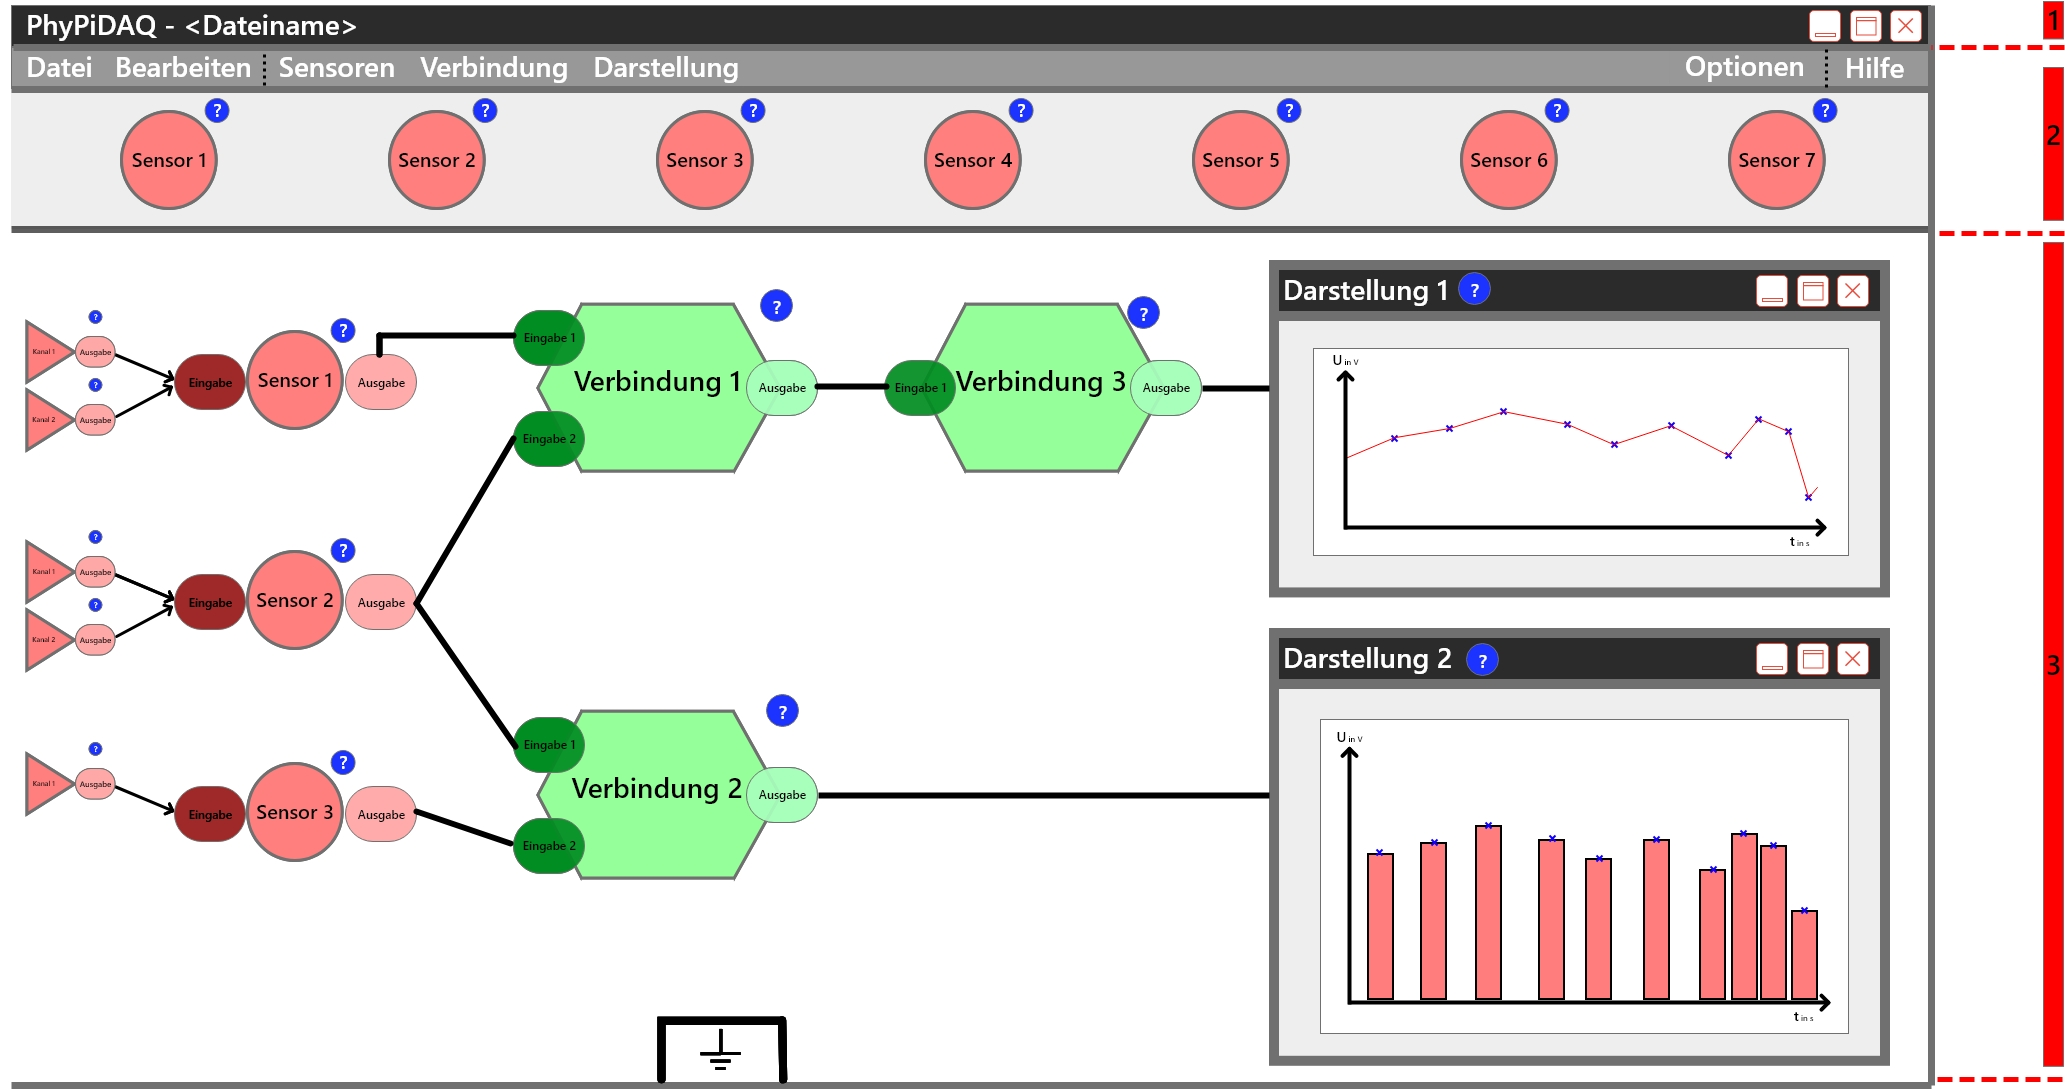
\includegraphics[width = 12cm]{Grafik/GUI-mit-Segmenten.jpg}
		\caption{Der Grundlegende Aufbau der Hauptbenutzeroberfl"ache}
		\label{GUI_Grundlage}
	\end{center}
\end{figure}

Abbildung 1 zeigt den Aufbau der Grafischen Benutzeroberfl"ache. Dabei geben die Zahlen in den roten K"astchen, rechts von dem Hauptfenster, die logische Unterteilung an.

Die zu dem jeweiligen Teil gehörenden Elemente sollen im folgenden erkl"art werden.

\subsection{Die einzelnen Teile}

\subsubsection{Systemmen"uleiste}

\begin{tabular}[t]{p{1cm} p{10cm}}
	\vspace{0cm}
\includegraphics[width = 1 cm]{Grafik/PhyPiDAQ.jpg} & Der Name des Programmes wird hier angezeigt. Rechts daneben steht, sofern vorhanden, der Name der Datei, die gerade ge"offnet ist.\newline\\
	\vspace{0cm}
\includegraphics[width = 1 cm]{Grafik/Maximieren.jpg} & Das ''Maximieren''-Symbol vergrößert das Programmfenster auf die maximale Größe. Die Größe ist von der Benutzungsumgebung abh"angig.\newline\\
	\vspace{0cm}
\includegraphics[width = 1 cm]{Grafik/Minimieren.jpg} & Das ''Minimieren''-Symbol blendet das Programmfenster aus. Es ist weiterhin ge"offnet und wieder aufrufbar. \\
	\vspace{0cm}\includegraphics[width = 1 cm]{Grafik/Schließen.jpg} & Das ''Schliessen''-Symbol beendet die Anwendung. Vor dem Beenden findet eine Abfrage statt, ob der Anwender eventuell vorgenommene "Anderungen speichern m"ochte.\newline\\
\end{tabular}

\subsubsection{Auswahl}

\begin{tabular}[t]{p{1cm} p{10cm}}
	\vspace{0cm}
\includegraphics[width = 1 cm]{Grafik/Datei.jpg} & Unter dem Reiter ''Datei'' finden sich Optionen, die sich auf Dateien beziehen. Die wichtigsten sind: 
	\begin{itemize} 
		\item Das anlegen einer neuen Datei
		\item Das Speichern der aktuellen Datei
		\item Das "Offnen einer bereits erstellten Datei
	\end{itemize}\\
	\vspace{0cm}
\includegraphics[width = 1 cm]{Grafik/Bearbeiten.jpg} & Unter dem Reiter ''Bearbeiten'' finden sich Optionen, die das Ändern von Inhalten der aktuell ge"offneten Datei erm"oglichen. Die wichtigsten sind:
	\begin{itemize} 
		\item Das Kopieren eines ausgewählten Objektes
		\item Das Einfügen eines gespeicherten Objektes
		\item Das Anpassen eines ausgewälten Elements. Diese Einstellungsm"oglichkeiten sind von dem Objekt abhängig.
	\end{itemize}\\
	\vspace{0cm}
\includegraphics[width = 1 cm]{Grafik/Sensor.jpg} & ToDO\\
	\vspace{0cm}
\includegraphics[width = 1 cm]{Grafik/Verbindung.jpg} & ToDO\\
	\vspace{0cm}
\includegraphics[width = 1 cm]{Grafik/Dartstellung.jpg} & ToDO\\
	\vspace{0cm}
\includegraphics[width = 1 cm]{Grafik/Optionen.jpg} & ToDO\\
	\vspace{0cm}
\includegraphics[width = 1 cm]{Grafik/Hilfe.jpg} & ToDO\\
\end{tabular}

\subsubsection{Hauptfeld}

\begin{tabular}[t]{p{1cm} p{10cm}}
	\vspace{0cm}
\includegraphics[width = 1 cm]{Grafik/Information.jpg} & Das ''Informations''-Symbol zeigt nach einem Click weiterführende Informationen zu dem Element an, zu dem es geh"ort. So würde beispielsweise bei Verknüpfung die Funktion angezeigt werde, die sie realisiert.\newline\\
	\vspace{0cm}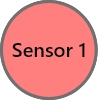
\includegraphics[width = 1 cm]{Grafik/Sensorelement.jpg} & ToDO\\
	\vspace{0cm}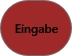
\includegraphics[width = 1 cm]{Grafik/Eingabe-Sensor.jpg} & ToDO\\
	\vspace{0cm}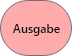
\includegraphics[width = 1 cm]{Grafik/Ausgabe-Sensor.jpg} & ToDO\\
	\vspace{0cm}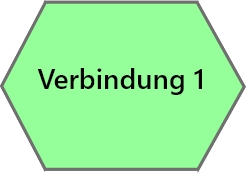
\includegraphics[width = 1 cm]{Grafik/Verbindungselement.jpg} & ToDO\\
	\vspace{0cm}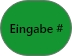
\includegraphics[width = 1 cm]{Grafik/Eingabe-Verbindung.jpg} & ToDO\\
	\vspace{0cm}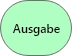
\includegraphics[width = 1 cm]{Grafik/Ausgabe-Verbindung.jpg} & ToDO\\
	\vspace{0cm}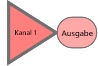
\includegraphics[width = 1 cm]{Grafik/Kanal.jpg} & ToDO\\
	\vspace{0cm}
\includegraphics[width = 1 cm]{Grafik/Verbindungspfeil.jpg} & ToDO\\
\end{tabular}

\subsection{Erweiterungsm"oglichkeiten}

\section{Spezielle Anforderungen an die Entwicklungsumgebung}

\section{Zeit- und Ressourcenplanung}

\begin{tabular}{| l | l | l |}
	\hline
	\textbf{Phase} & \textbf{Verantwortlicher} & \textbf{Zeitraum} \\ \hline
	Pflichtenheft & Jan Küblbeck & KW 20–22 \\
	Entwurf & Leon Huck & KW 23–26 \\
	Implementierung & Stefan Geretschläger & KW 27–29, 31 \\
	Klausurenphase & — & KW 30, 32 \\
	Qualitätssicherung & David Gawron & KW 33–35 \\
	Abnahme & — & KW 36 \\
	Abschlussprüfung & Linus Ruhnke & KW 37/38 \\
	\hline
\end{tabular}

\subsection{Entwurfsphase}

\subsection{Implementierungsphase}

\section{Ergänzungen}

\section{Glossar}

\renewcommand*{\glossarysection}[2][]{}	% prevents double glossary section heading
\printnoidxglossaries				% generate pdf twice when adding new entries


\end{document}